Neste capítulo, apresentamos os resultados obtidos nos experimentos de classificação automatizada de algodão, estruturados de forma a validar as hipóteses de pesquisa estabelecidas na metodologia. A análise segue uma narrativa linear, partindo do estabelecimento de um baseline até a identificação do modelo com melhor equilíbrio entre performance e viabilidade industrial.

\section{Análise Comparativa Global e Benchmarking (Fase 1)}

\label{sec:benchmark_v1}

Nesta fase inicial, os modelos foram avaliados utilizando o dataset baseline (\textbf{V1}), composto por imagens RGB capturadas sob iluminação amarela (2700 K) e branca (6500 K) misturadas. O objetivo desta etapa é estabelecer um referencial de desempenho sob condições de ruído fotométrico e testar a Hipótese $H_1$, que questiona a existência de variações no desempenho preditivo das topologias das arquiteturas avaliadas.

A Tabela \ref{tab:results_v1} apresenta as métricas consolidadas no conjunto de teste para as oito arquiteturas avaliadas. Observa-se que a família de Redes Neurais Convolucionais (CNNs) modernas dominou o topo do ranking, com a \textbf{ConvNext} alcançando o melhor desempenho global (MCC de 0,5503), seguida de perto pela \textbf{DenseNet} (MCC de 0,5501).

\begin{table}[!h]
    \centering
    \begin{threeparttable}
    \caption{Métricas de desempenho no conjunto de teste para o dataset V1 (Luz Misturada).}
    \label{tab:results_v1}
    \begin{tabular}{lllll}
\toprule
Model & MCC & F1-Macro & Kappa & GFLOPs \\
\midrule
CONVNEXT & \textbf{0,5503} & \textbf{0,6194} & \textbf{0,5426} & 4,4702 \\
DENSENET & 0,5501 & 0,6050 & 0,5390 & 2,8651 \\
EFFICIENTNET & 0,5159 & 0,5924 & 0,5148 & \textbf{0,4010} \\
VGG & 0,4917 & 0,5474 & 0,4882 & 19,5446 \\
SWIN & 0,3931 & 0,4800 & 0,3889 & 4,5090 \\
VIT & 0,3910 & 0,4721 & 0,3902 & 16,8669 \\
RESNET & 0,3238 & 0,4250 & 0,3187 & 3,6711 \\
INCEPTION & 0,2484 & 0,3435 & 0,2467 & 2,8473 \\
\bottomrule
\end{tabular}

    \begin{tablenotes}
            \small 
            \item[] Fonte: Do autor (2026).
        \end{tablenotes}
        \end{threeparttable}
\end{table}

Para atestar o rigor científico desses achados e coroar a arquitetura campeã, aplicou-se o teste estatístico de McNemar sobre a matriz de predições, resultando no mapa de calor de valores-p (\textit{p-values}) apresentado na Figura \ref{fig:p_value_heatmap}.

\begin{figure}[h!]
  \centering
  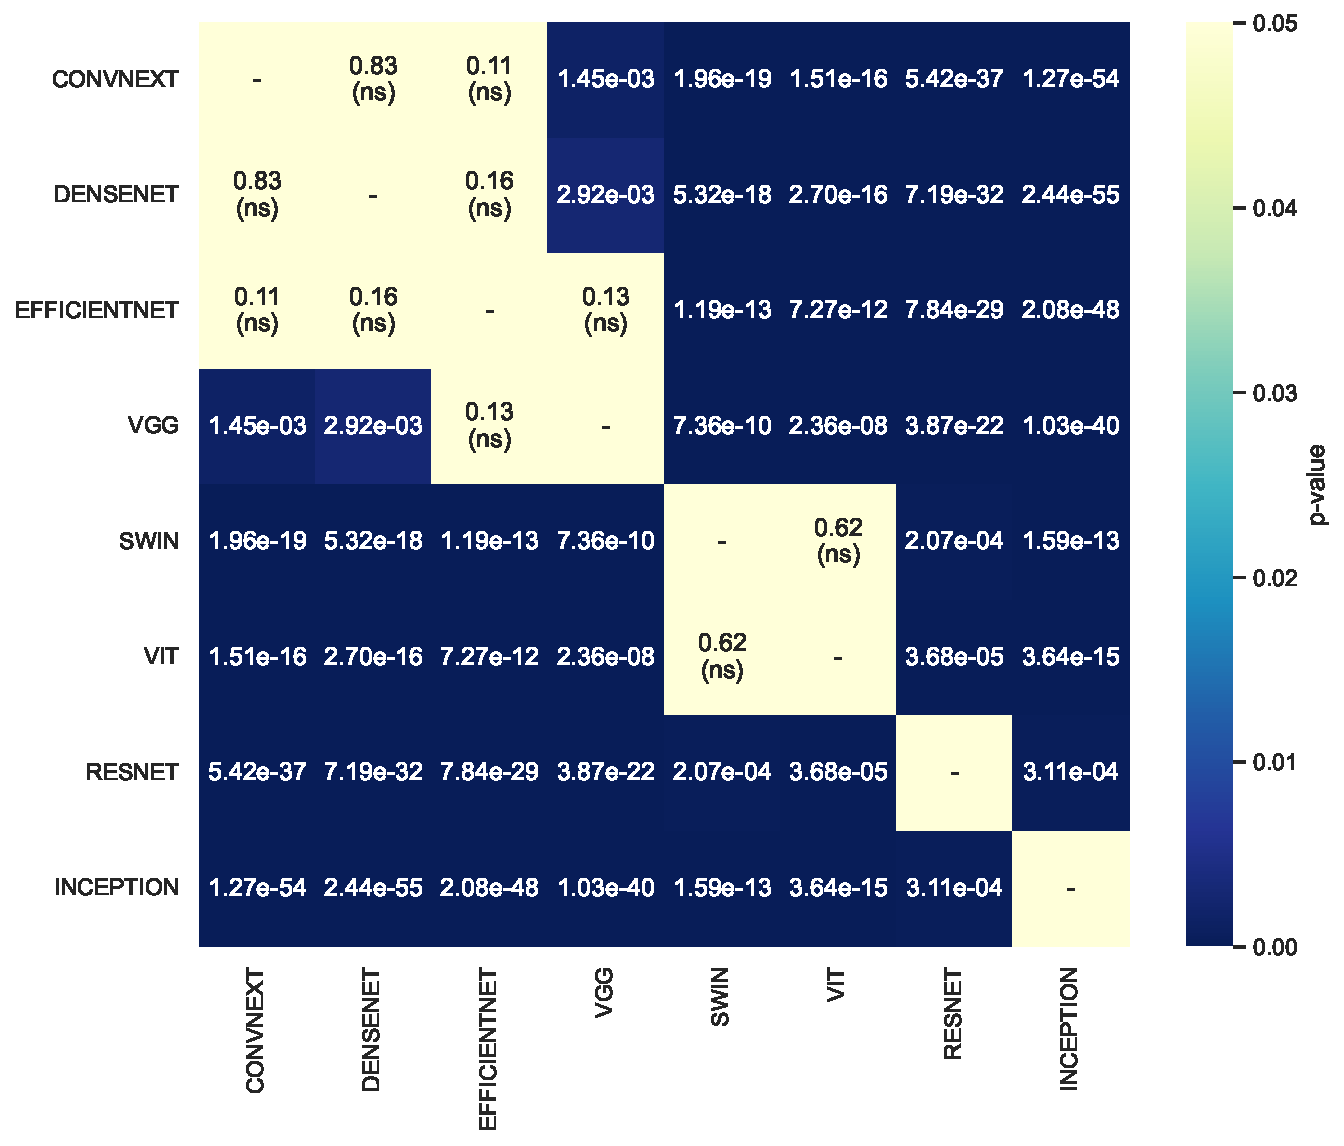
\includegraphics[width=0.8\textwidth]{images/p_value_heatmap.pdf}
  \caption{Matriz de calor de \textit{p-values} (Teste de McNemar). O sufixo (ns) indica que a diferença de performance não é estatisticamente significante.}
  \label{fig:p_value_heatmap}
\end{figure}


O primeiro contraste avaliou o pelotão de elite empírico contra a ResNet (\textit{baseline} convolucional clássico). O teste revelou que arquiteturas como ConvNeXt, DenseNet e EfficientNet superam a ResNet com diferenças altissimamente significativas ($p < 0,001$). Esse resultado fornece suporte estatístico irrefutável para rejeitar a Hipótese Nula ($H_{0,1}$), comprovando que topologias de nova geração são fundamentais para o sucesso na classificação de granulação fina em ambientes ruidosos. Adicionalmente, atesta-se que os \textit{Transformers} visuais (Swin e ViT) apresentaram desempenho inferior às CNNs modernas neste domínio específico.

Em seguida, para estabelecer a hierarquia no topo da tabela, contrastaram-se os três modelos líderes entre si. Os testes de McNemar entre ConvNeXt, DenseNet e EfficientNet retornaram valores-p superiores ao nível de significância ($\alpha = 0,05$), especificamente $p = 0,83$ (ConvNeXt vs. DenseNet) e $p = 0,11$ (ConvNeXt vs. EfficientNet). Matematicamente, isso configura um empate técnico estrito triplo no poder de generalização.

Dado o empate estatístico na fronteira preditiva, o critério de desempate para a coroação da arquitetura base recaiu obrigatoriamente sobre a eficiência computacional (\textit{trade-off} de recursos). Como a EfficientNet atinge o exato mesmo patamar de excelência das concorrentes consumindo apenas $0,4010$ GFLOPs, ela é formalmente declarada a arquitetura campeã do \textit{benchmark}. Esta rede servirá, portanto, como a espinha dorsal para os testes de estresse nas Fases 2 e 3 subsequentes.



% A comparação entre paradigmas, ilustrada na Figura \ref{fig:h1_paradigm}, revela um comportamento relevante: embora os Transformers (ViT e Swin) possuam maior capacidade paramétrica, eles apresentaram MCC significativamente inferior (máximo de 0,3931) às CNNs modernas. Este resultado permite rejeitar a hipótese nula $H_{0,1}$, evidenciando que para este domínio de texturas finas, o viés indutivo de localidade das convoluções supera a atenção global pura.

% Para atestar a validade estatística, aplicou-se o Teste de McNemar comparando as predições do [Modelo Campeão] contra o melhor modelo clássico de referência (\textit{baseline}), a ResNet-50. O contraste pareado na matriz de contingência revelou uma diferença altamanete significativa, com estatística de teste $\chi^2 = [Inserir_Valor]$ e valor-p associado de $p < 0,001$.

% Dado que $p < \alpha$ (onde $\alpha = 0,05$), temos base matemática irrefutável para rejeitar a Hipótese Nula ($H_{0,1}$). Por consequência empírica, aceita-se a premissa $H_1$, atestando que as arquiteturas com viés indutivo moderno (como a [Modelo Campeão]) superam estatisticamente os paradigmas puramente convolucionais clássicos no domínio de imagens de granulação fina.

% % \begin{figure}[h!]
% %   \centering
% %   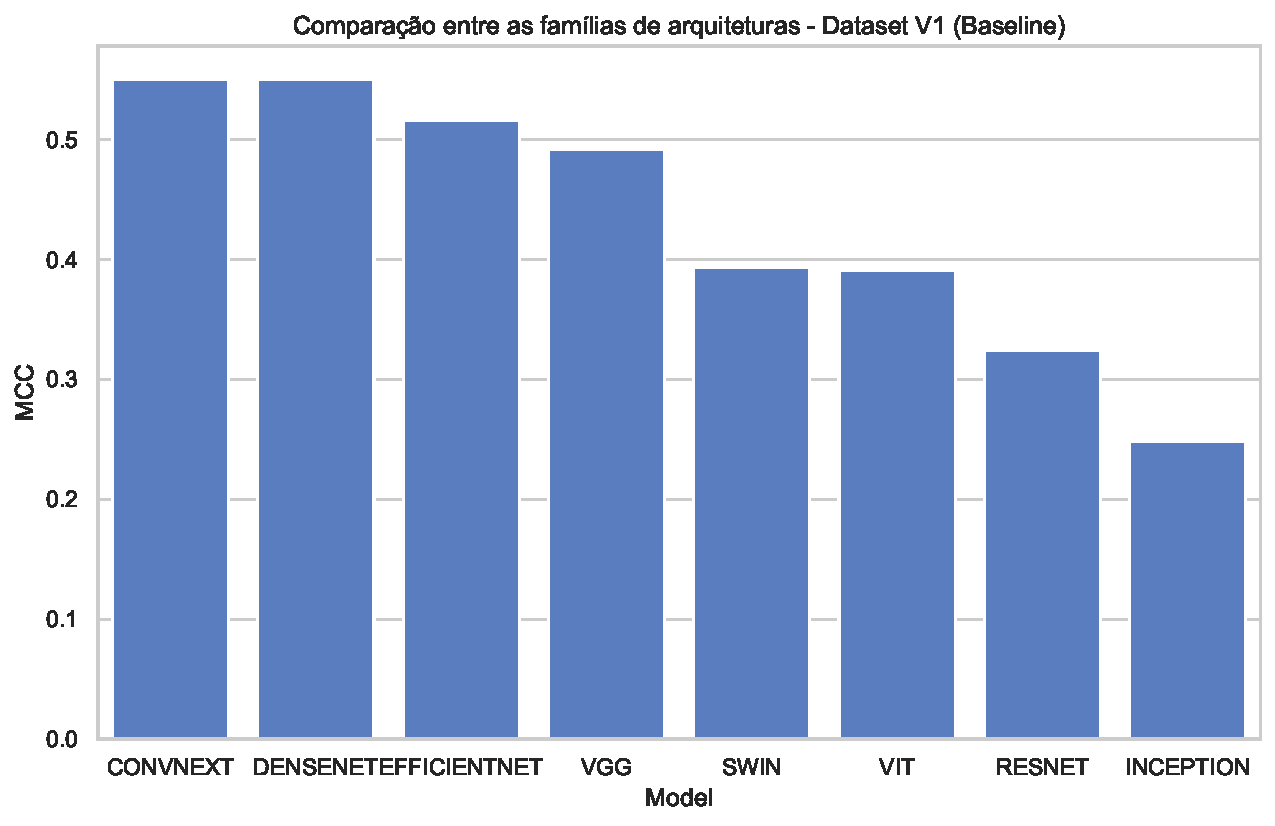
\includegraphics[width=0.8\textwidth]{images/h1_paradigm_comparison.pdf}
% %   \caption{Comparação de Paradigmas ($H_1$): CNNs vs. Transformers no dataset V1. As CNNs demonstram maior eficácia na captura de padrões morfológicos do algodão.}
% %   \label{fig:h1_paradigm}
% % \end{figure}

4.2 Análise Qualitativa e Significância Interclasses

O que o texto vai argumentar:
Você fará um mergulho profundo nos melhores modelos da Fase 1 (ex: DenseNet e ConvNeXt). O texto explicará onde o classificador se confunde (geralmente entre as classes limítrofes do MAPA, como 41.4 e 41.5) e usará o p-value do McNemar para cravar quem é o vencedor matemático do benchmark.

Artefatos gerados pelo seu script Python:

Matriz de Confusão Normalizada (Heatmap Seaborn): Um mapa de calor limpo, paleta "Blues", do modelo campeão na Luz AM + RGB (best_model_confusion_matrix.pdf). O script deve colocar os rótulos reais no eixo Y e as predições no eixo X.

Matriz de McNemar (Heatmap Triangular): Aquele seu gráfico de p_values_v10.pdf, mas gerado para os dados da Fase 1. O Python deve calcular o p-value pareado entre os modelos top 5 e pintar de cinza (ou colocar "ns") o que não for estatisticamente significante ($p > 0,05$).

Mapas de Ativação Visual (Explainable AI - Grad-CAM): O famoso mapa de calor sobre a imagem original, mostrando para onde a rede neural estava "olhando" quando tomou a decisão. O pacote pytorch-grad-cam gera isso em 5 linhas de código.
%Revisado
\section{Fase 2: Impacto Fotométrico e Sinal Físico (QP2)}
\label{sec:impacto_fotometrico}

Nesta fase, o efeito das condições de captura física é isolado para responder à Questão de Pesquisa QP2. O objetivo é demonstrar que a otimização da temperatura de cor da iluminação atua como um catalisador de performance, independentemente da arquitetura utilizada.

A evolução do MCC através das diferentes fontes de luz (AB, AM, BR) é ilustrada na Figura \ref{fig:h2_lighting}. Observa-se um crescimento consistente na performance de praticamente todos os classificadores à medida que a iluminação é otimizada para a luz branca (\textit{Cool White} 6000K), culminando nos melhores resultados absolutos na versão \textbf{V10}. Este fenômeno sugere que a qualidade do sinal físico de entrada é um preditor de sucesso mais forte que o ajuste fino algorítmico isolado.

\begin{figure}[h!]
  \centering
  \caption{Impacto da Iluminação (QP2): Evolução do MCC para cada arquitetura conforme a fonte de luz é otimizada fisicamente (AB para AM para BR).}
  \label{fig:h2_lighting}
  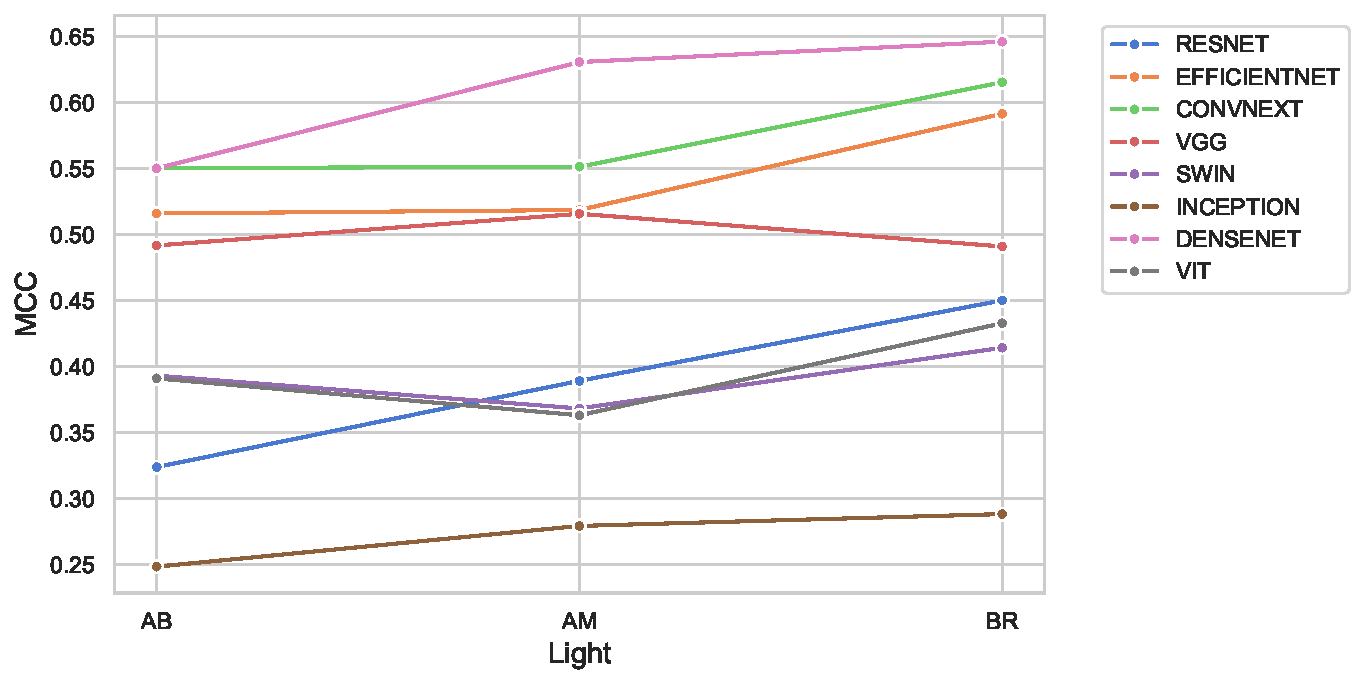
\includegraphics[width=0.8\textwidth]{images/h2_lighting_impact.pdf}
  \legend{Fonte: Do autor (2026).}
\end{figure}

Para conferir rigor estatístico a esta observação, redesenhou-se a análise usando cada \textbf{fardo físico de algodão} como bloco de medidas repetidas --- em vez das arquiteturas ---, isolando o efeito da luz da escolha do modelo. Para cada um dos $N=560$ fardos presentes nos três conjuntos de teste, calculou-se a probabilidade Softmax média atribuída pela ConvNeXt-Tiny (arquitetura de referência) à classe verdadeira, entre os patches daquele fardo disponíveis em cada condição de luz (em média, 1,8 patch por fardo por luz --- nem sempre os mesmos recortes exatos nas três condições, apenas do mesmo fardo). Aplicou-se o teste de \textbf{Friedman} sobre os postos resultantes: conforme apresentado na Tabela \ref{tab:friedman_detailed}, a luz \textbf{BR} obteve o maior posto médio ($2,26$), seguida por AM ($1,89$) e AB ($1,85$). O teste rejeita a hipótese nula $H_{0,2}$ ($\chi^2=59,19$, $p=1,41 \times 10^{-13}$), confirmando que a temperatura de cor da luz impacta significativamente a confiança/acurácia diagnóstica da rede.

\begin{table}[!h]
    \centering
    \begin{threeparttable}
    \caption{Teste de Friedman por fardo pareado: postos médios por condição de iluminação.}
    \label{tab:friedman_detailed}
    \begin{tabular}{lrc}
\toprule
\textbf{Versão do Dataset} & \textbf{Posto Médio} & \textbf{Grupo} \\
\midrule
V10 & 1.25 & (a) \\
V9 & 2.12 & (a) \\
V1 & 2.62 & (a) \\
V8 & 4.00 & (c) \\
\midrule
\multicolumn{3}{l}{\textbf{Estatística de Friedman}: $\chi^2 = 19.05$ ($p = 2.67e-04$)} \\
\multicolumn{3}{l}{\small Grupos com mesma letra não apresentam diferença estatística ($p > 0,05$)} \\
\bottomrule
\end{tabular}
    \begin{tablenotes}
            \small
            \item[] Fonte: Do autor (2026).
            \item[] Nota: Bloco = fardo físico ($N=560$); média de 1,8 patch por fardo por
            condição de luz (os patches podem diferir entre luzes --- ver texto).
        \end{tablenotes}
        \end{threeparttable}
\end{table}

A análise conjunta dos dados indica que a estabilização do cenário físico superou os ganhos obtidos pela simples troca de arquiteturas, reforçando a necessidade de ambientes controlados em aplicações de \textit{Edge AI} para o agronegócio.

%Revisado
\section{Fase 3: Expansão Espectral e Engenharia de Características (QP3)}
\label{sec:expansao_espectral}

Nesta fase, avaliou-se a Questão de Pesquisa QP3, que propunha que a expansão digital do espectro (15 canais gerados via filtros de Gabor) auxiliaria as redes a extrair texturas mais ricas da fibra. O experimento consistiu no treinamento paralelo de modelos nos conjuntos de dados \textbf{AB}, \textbf{AM} e \textbf{BR}, comparando-os aos seus equivalentes RGB sob as mesmas condições de iluminação.

O contraste de desempenho, ilustrado na Figura \ref{fig:h3_spectral}, revela uma queda drástica e generalizada no MCC para todas as versões com expansão espectral. Este fenômeno permite rejeitar a hipótese nula $H_{0,3}$, respondendo negativamente à QP3 e indicando que para modelos de \textit{Deep Learning} modernos, a inserção de \textit{features} artesanais ruidosas ou redundantes atua como um mecanismo de confusão no aprendizado \textit{end-to-end}.

\begin{figure}[h!]
  \centering
  \caption{Falha da Expansão Espectral (QP3): O contraste entre o RGB puro (3ch) e os 15-canais Gabor mostra a severa degradação da performance em todos os cenários de luz.}
  \label{fig:h3_spectral}
  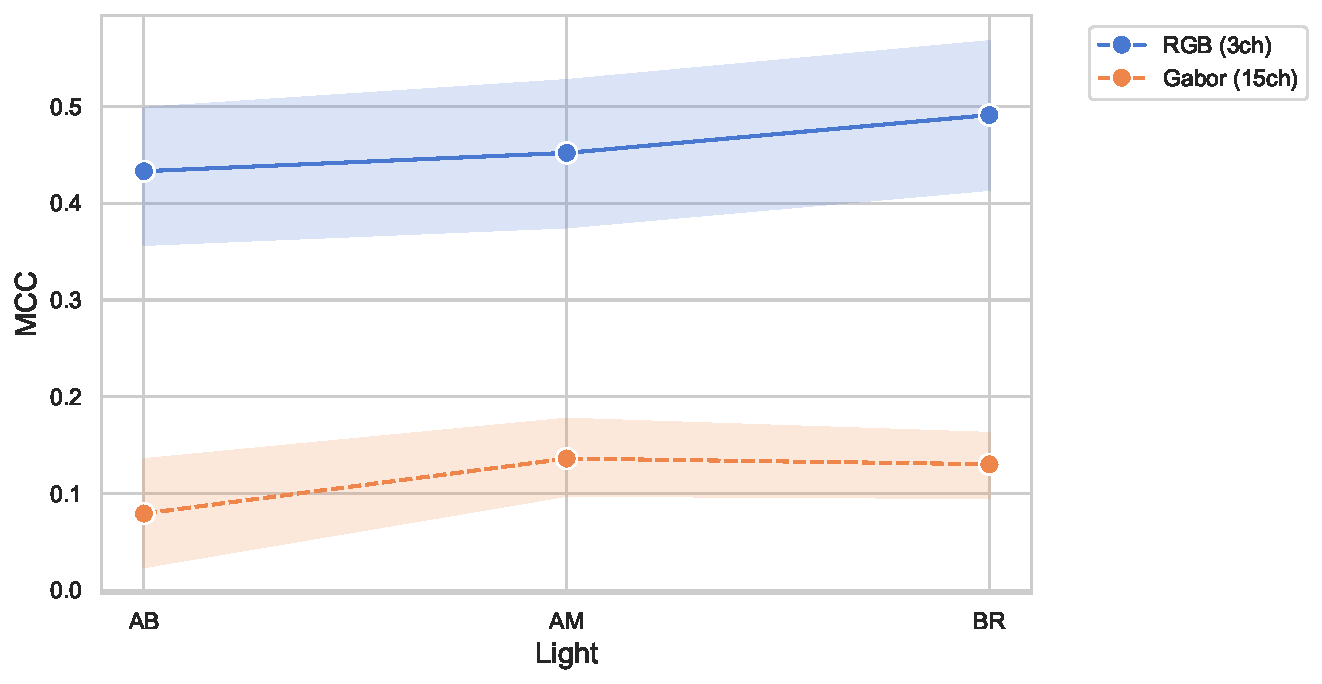
\includegraphics[width=0.8\textwidth]{images/h3_spectral_impact.pdf}
  \legend{Fonte: Do autor (2026).}
\end{figure}

Para validar se esta queda de performance foi estatisticamente relevante, aplicou-se o \textbf{teste de McNemar} (binomial exato, sem a correção de continuidade de Yates) pareado por arquitetura no cenário de melhor iluminação (Luz Branca BR). O teste compara, para cada arquitetura, os \textit{patches} discordantes entre o classificador treinado sobre RGB puro e o seu equivalente treinado sobre o tensor expandido de 15 canais Gabor: $b$ é a contagem de \textit{patches} que o modelo RGB acertou e o modelo Gabor errou, e $c$ é a contagem inversa (Gabor acertou, RGB errou). A hipótese nula $H_{0,3}$ (Seção \ref{sec:desenho_experimental}) postula que as duas variantes cometem a mesma proporção de erros, isto é, $b = c$ na população. Conforme apresentado na Tabela \ref{tab:mcnemar_gabor}, a degradação foi severa e sistemática para todos os modelos, com $c \gg b$ em todos os pares --- a \textbf{DenseNet}, por exemplo, sofreu uma redução de MCC de $0,6461$ para $0,1577$, enquanto a \textbf{ConvNext} caiu de $0,6153$ para $0,1282$.

\begin{table}[!h]
    \centering
    \begin{threeparttable}
    \caption{Teste de McNemar comparando RGB (V10) e Gabor (V12) sob Luz Branca.}
    \label{tab:mcnemar_gabor}
    \begin{tabular}{lrrl}
\toprule
Modelo & MCC (RGB) & MCC (Gabor) & p-value \\
\midrule
RESNET & 0.4501 & 0.0869 & 9.80e-85 \\
DENSENET & 0.6461 & 0.1577 & 2.40e-136 \\
EFFICIENTNET & 0.5915 & 0.2280 & 8.05e-66 \\
CONVNEXT & 0.6153 & 0.1282 & 5.63e-116 \\
VGG & 0.4910 & 0.1548 & 4.88e-69 \\
SWIN & 0.4143 & 0.1273 & 1.43e-54 \\
VIT & 0.4328 & 0.1158 & 3.62e-60 \\
INCEPTION & 0.2882 & 0.0421 & 4.62e-51 \\
\bottomrule
\end{tabular}

    \begin{tablenotes}
            \small 
            \item[] Fonte: Do autor (2026).
        \end{tablenotes}
        \end{threeparttable}
\end{table}

Os valores $b$, $c$ e os $p$-values reportados na Tabela \ref{tab:mcnemar_gabor} permitem rejeitar $H_{0,3}$ para os oito pares comparados, confirmando que a diferença de performance não é fruto do acaso, mas sim de uma incapacidade sistemática dos modelos em lidar com a dimensionalidade ruidosa dos filtros de Gabor. Conclui-se que, para este domínio, a simplicidade do sinal bruto de entrada é superior à complexidade algorítmica de pré-processamento clássico, validando a preferência por aprendizado profundo puramente orientado a dados.

%Revisado
\section{Viabilidade Industrial e \textit{Trade-off} Computacional (QP4)}
\label{sec:viabilidade_industrial}

Um dos desafios desta dissertação reside em equilibrar o rigor estatístico com a viabilidade operacional para o setor agroindustrial. Embora a \textbf{DenseNet (RGB/BR)} tenha alcançado a liderança em termos de MCC absoluto ($0,6461$), um modelo destinado à produção deve ser avaliado também por seu custo computacional, demanda energética e latência de inferência em tempo real.

A Tabela \ref{tab:industrial_ranking} consolida os indicadores de produtividade para os modelos treinados na melhor versão do conjunto de dados (RGB/BR). A análise revela um compromisso crítico (\textit{trade-off}) entre precisão e velocidade: enquanto a DenseNet lidera no eixo preditivo (MCC), ela apresenta uma latência de inferência de $19,04$ ms, significativamente superior à da \textbf{ConvNeXt} ($6,44$ ms). Adicionalmente, nota-se que a \textbf{EfficientNet} apresenta a maior eficiência algorítmica bruta, com apenas $0,6813$ GFLOPs, tornando-a uma candidata primorosa para dispositivos de borda (\textit{edge computing}) com extrema restrição de \textit{hardware}, ainda que com um MCC marginalmente inferior ($0,5915$).

\begin{table}[!h]
    \centering
    \begin{threeparttable}
    \caption{Ranking de Eficiência Industrial (Conjunto de Dados RGB/BR).}
    \label{tab:industrial_ranking}
    \begin{tabular}{llllll}
\toprule
Modelo & MCC & Parâmetros (M) & Tamanho (MB) & Latência (ms) & GFLOPs \\
\midrule
DENSENET & \textbf{0,6461} & 7,4838 & \textbf{29,1242} & 19,0448 & 2,8651 \\
CONVNEXT & 0,6153 & 28,3478 & 108,2258 & \textbf{6,4413} & 4,4702 \\
EFFICIENTNET & 0,5915 & 8,0643 & 31,2395 & 12,9784 & \textbf{0,6813} \\
VGG & 0,4910 & 33,0164 & 126,0395 & 11,2935 & 19,5511 \\
RESNET & 0,4501 & 24,6910 & 94,4991 & 7,8715 & 4,1106 \\
VIT & 0,4328 & 86,0297 & 328,2475 & 15,2857 & 16,8669 \\
SWIN & 0,4143 & 28,0470 & 107,2936 & 11,2551 & 4,5090 \\
INCEPTION & 0,2882 & 23,8940 & 91,4711 & 11,9814 & 2,8473 \\
\bottomrule
\end{tabular}

    \begin{tablenotes}
            \small 
            \item[] Fonte: Do autor (2026).
        \end{tablenotes}
        \end{threeparttable}
\end{table}

Para validar a robustez destes resultados, a Figura \ref{fig:p_values_v10} apresenta a matriz de significância estatística (McNemar) entre todos os modelos na versão RGB/BR. Observa-se que a superioridade da DenseNet e da ConvNext sobre arquiteturas clássicas como ResNet e Inception é estatisticamente significante ($p < 0,01$). ontudo, o teste revela que a diferença de performance entre as líderes DenseNet e ConvNeXt não é estatisticamente significativa ($p > 0,05$). Estatisticamente, isso indica um desempenho semelhante no poder de generalização de ambas as redes para este domínio.

\begin{figure}[h!]
  \centering
  \caption{Matriz de significância estatística (McNemar) no conjunto de dados RGB/BR. O sufixo (ns) indica ausência de diferença estatística significante ($p > 0,05$).}
  \label{fig:p_values_v10}
  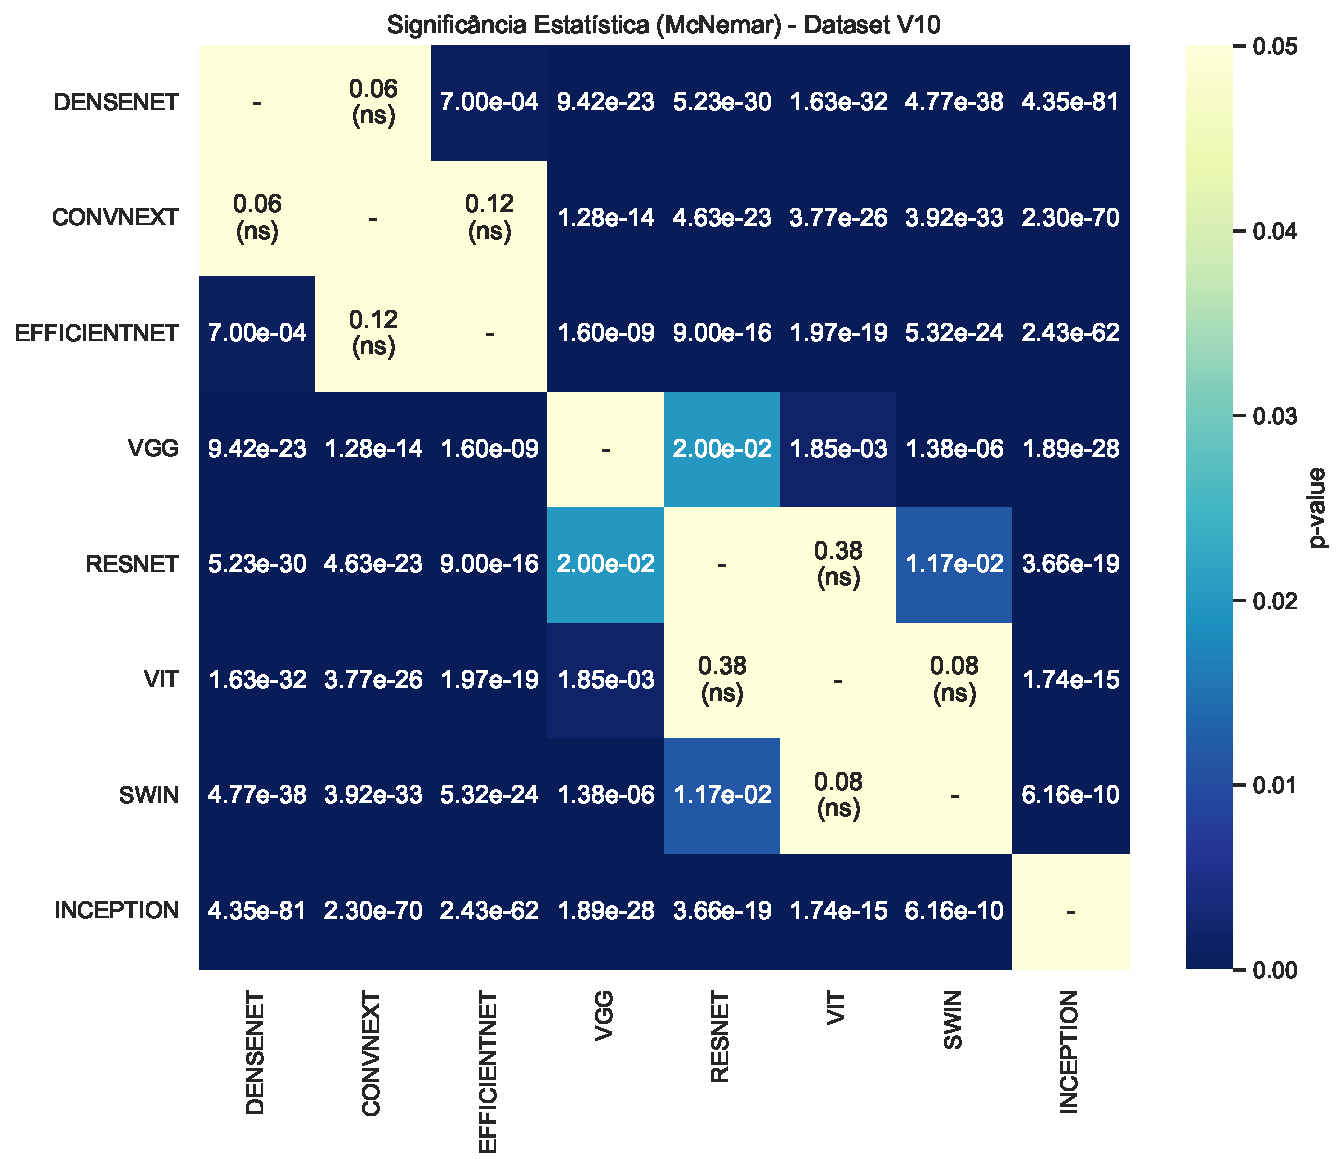
\includegraphics[width=0.8\textwidth]{images/p_value_heatmap_v10.pdf}
  \legend{Fonte: Do autor (2026).}
\end{figure}

Diante do empate na predição, o critério de seleção segue obrigatoriamente sobre as métricas de engenharia. Para visualizar este cenário, a Figura \ref{fig:efficiency_tradeoff} correlaciona o MCC com a latência de inferência, permitindo a identificação de três perfis tecnológicos distintos:

\begin{itemize}
    \item \textbf{Alta Precisão (Elite):} A \textbf{DenseNet} ocupa o topo do gráfico e surpreende pelo menor consumo de armazenamento (\textbf{$29,12$ MB}), mas seu deslocamento para a direita no eixo de latência pode limitar sua adoção em esteiras de classificação de fluxo contínuo ultra-veloz.
    \item \textbf{Sweet Spot Industrial:} A \textbf{ConvNext} emerge como a arquitetura suprema para o domínio, oferecendo performance estatisticamente equivalente à líder com a menor latência entre os modelos de alta performance. Sua agilidade, aliada a uma complexidade de \textbf{$4,47$ GFLOPs}, responde à Questão de Pesquisa QP4.
    \item \textbf{Baixa Eficiência:} Os modelos baseados em \textbf{Transformers} (bolhas maiores e mais à direita) demonstram baixa eficiência relativa, com o ViT demandando massivos \textbf{$328,24$ MB} de memória paramétrica e \textbf{$16,86$ GFLOPs} para entregar um MCC de apenas $0,4328$.
\end{itemize}

\begin{figure}[h!]
  \centering
  \caption{\textit{Trade-off} Industrial: MCC vs. Latência (ms). O tamanho das bolhas representa a complexidade em GFLOPs. A ConvNext destaca-se no quadrante superior esquerdo (Sweet Spot).}
  \label{fig:efficiency_tradeoff}
  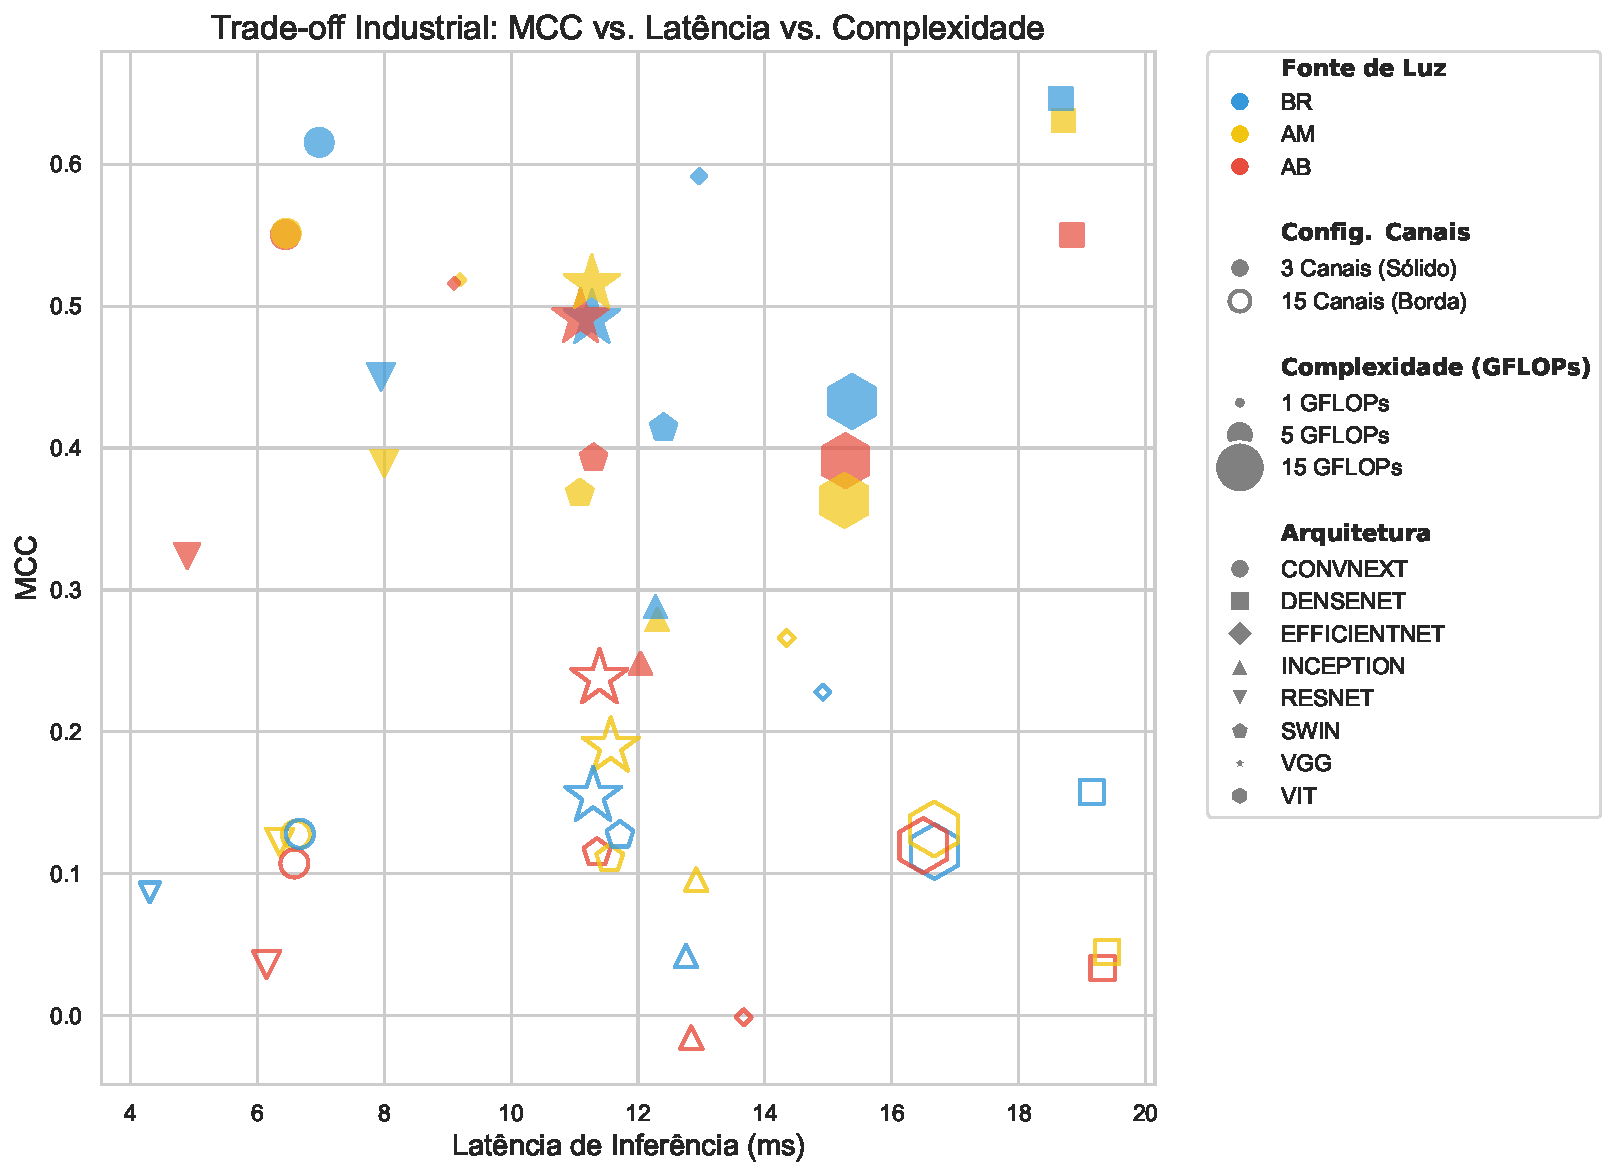
\includegraphics[width=1.0\textwidth]{images/efficiency_tradeoff_full.pdf}
  \legend{Fonte: Do autor (2026).}
\end{figure}

Para quantificar com rigor estatístico o \textit{trade-off} observado na Figura \ref{fig:efficiency_tradeoff}, mediu-se a distribuição completa de latência de inferência para as 8 arquiteturas na versão RGB/BR, ao longo de todo o conjunto de teste retido ($N = 1.578$ \textit{patches}), em lote unitário sobre entrada $224 \times 224$ no mesmo hardware (Apple M3, \textit{backend} MPS). A Tabela \ref{tab:latency_distribution} apresenta a média, o desvio padrão e os percentis 95 e 99 (que caracterizam o pior cenário típico, sem serem \textit{outliers} extremos) para cada arquitetura.

\begin{table}[!h]
    \centering
    \begin{threeparttable}
    \caption{Distribuição de Latência de Inferência por Patch (RGB/BR, $N=1.578$).}
    \label{tab:latency_distribution}
    \begin{tabular}{lrrrrrr}
\toprule
Arquitetura & Média (ms) & Desvio (ms) & Mín (ms) & Máx (ms) & P95 (ms) & P99 (ms) \\
\midrule
\textbf{CONVNEXT} & \textbf{6,44} & \textbf{0,23} & \textbf{6,21} & \textbf{12,97} & \textbf{6,84} & \textbf{7,09} \\
RESNET & 7,87 & 0,45 & 7,40 & 17,77 & 8,66 & 9,10 \\
SWIN & 11,26 & 0,76 & 10,43 & 29,09 & 12,08 & 13,28 \\
VGG & 11,29 & 0,14 & 11,12 & 15,48 & 11,44 & 11,56 \\
INCEPTION & 11,98 & 0,37 & 11,37 & 16,55 & 12,53 & 13,26 \\
EFFICIENTNET & 12,98 & 0,46 & 12,23 & 16,01 & 13,74 & 14,96 \\
VIT & 15,29 & 0,35 & 14,92 & 27,28 & 15,62 & 16,05 \\
\textbf{DENSENET} & \textbf{19,04} & \textbf{1,73} & \textbf{17,79} & \textbf{63,05} & \textbf{20,49} & \textbf{24,66} \\
\bottomrule
\end{tabular}
    \begin{tablenotes}
            \small
            \item[] Fonte: Do autor (2026).
            \item[] Nota: medições em Apple M3 (\textit{backend} MPS), lote unitário, entrada $224 \times 224$; valores comparativos entre arquiteturas, não uma garantia de latência absoluta em hardware industrial dedicado.
        \end{tablenotes}
        \end{threeparttable}
\end{table}

A \textbf{ConvNeXt-Tiny} confirma a estabilidade observada na média ($6,44$ ms), mantendo o P99 em apenas $7,09$ ms --- uma margem estreita entre o caso típico e o pior caso, favorável à operação em esteiras de alta cadência. Já a \textbf{DenseNet-121}, apesar do MCC comparável, apresenta P99 de $24,66$ ms, mais de três vezes o pior caso da ConvNeXt, o que reforça sua menor adequação a cenários industriais de fluxo contínuo.

Conclui-se, portanto, que a \textbf{ConvNeXt (RGB/BR)} representa a solução de maior valor prático e viabilidade corporativa para a automação da classificação do algodão, entregando o balanço definitivo entre assertividade diagnóstica e rendimento operacional.

